% vim: set tw=78 sts=2 sw=2 ts=8 aw et ai:
\documentclass[conference]{IEEEtran}

\usepackage{ucs}
\usepackage[utf8x]{inputenc}
\usepackage[english]{babel}
%\usepackage{hyperref}	  % use \url{http://$URL} or \href{http://$URL}{Name}
\usepackage{underscore}	  % underscores need not be escaped
\usepackage{subfigure}
\usepackage{verbatim}
\usepackage{float}

% Support for including graphics
\usepackage{graphicx}
\DeclareGraphicsExtensions{.pdf,.png,.jpg}

\begin{document}

\title{Steganographic Access Control Using TCP/IP Headers}

\author{\IEEEauthorblockN{Silviu Petria, Silviu Popescu,
                          Valeriu Stanciu, Radu Stancu}
\IEEEauthorblockA{Automatic Control and Computers Faculty\\
Politehnica University of Bucharest\\
Emails: silviu.petria@gmail.com, silviupopescu1990@gmail.com,
valeriudanielstanciu@yahoo.com, stancumradu@gmail.com}}

\maketitle

\begin{abstract}
% vim: set tw=78 sts=2 sw=2 ts=8 aw et ai:
Insert abstract here.

\end{abstract}

%\textbf{\textit{Keywords -- ala, bala, portocala}}

\begin{IEEEkeywords}
Steganography, Security, TCP/IP Headers, Covert channels
\end{IEEEkeywords}

%\IEEEpeerreviewmaketitle

\section{Introduction}
\label{sec:introduction}
% vim: set tw=78 sts=2 sw=2 ts=8 aw et ai:

Steganography is the science of encoding messages in such a way that only the
sender and receiver can read them. It’s different from cryptography in the
sense that you don’t actually encode the message with a key or an algorithm,
instead hiding the message in things like images (each letter in a pixel, far
from each other enough so it doesn’t raise suspicion), audio files (a certain
tone at a certain interval can signify a letter) and even plain text
(repetition of certain letters can translate into a hidden message).

Although steganography has been used as early as Ancient Greece, the constant
development of technology has spawned a new field of research, namely digital
steganography. This focuses more on applying steganography in sending messages
over a network, either for increased security (plain cryptography can be
cracked if the attacker figures out what type of encryption you are using),
or for sending messages in such a way the network administrator is unaware
of them (for trivial tasks that would otherwise cost the user money, e.g. in a
cloud environment).

The purpose of this paper is to offer a solution for hiding messages in the
TCP/IP header. We aim to offer both a decent amount of space to store the
message and an encoding that will minimize the size of the message.


\section{Architecture}
\label{sec:architecture}
% vim: set tw=78 sts=2 sw=2 ts=8 aw et ai:

Our framework consists of a client and a server which are aware of the exact
encoding scheme used by our steganographic approach. Both the client and the
server have submodules responsible for a category of functions.

The client consists of 3 components: I/O, Codec and Net as outlined in Figure
\ref{fig:architecture}. The I/O module is responsible for capturing user input
before passing it to the encoding phase and retrieving server output from the
decoding phase. The Codec block splits the input in chunks suitable for sending
in a single packet from the client to the server and extracts chunks from
incoming packets sent by the server. The last outgoing chunk of any user input
or server response is marked with a special byte sequence. Last but not least,
the Net module handles network communication. Its purpose is to create a dummy
packet which has seemingly relevant data, but which contains the information of
interest in the options field of the TCP Header.

\begin{figure}
  \centering
  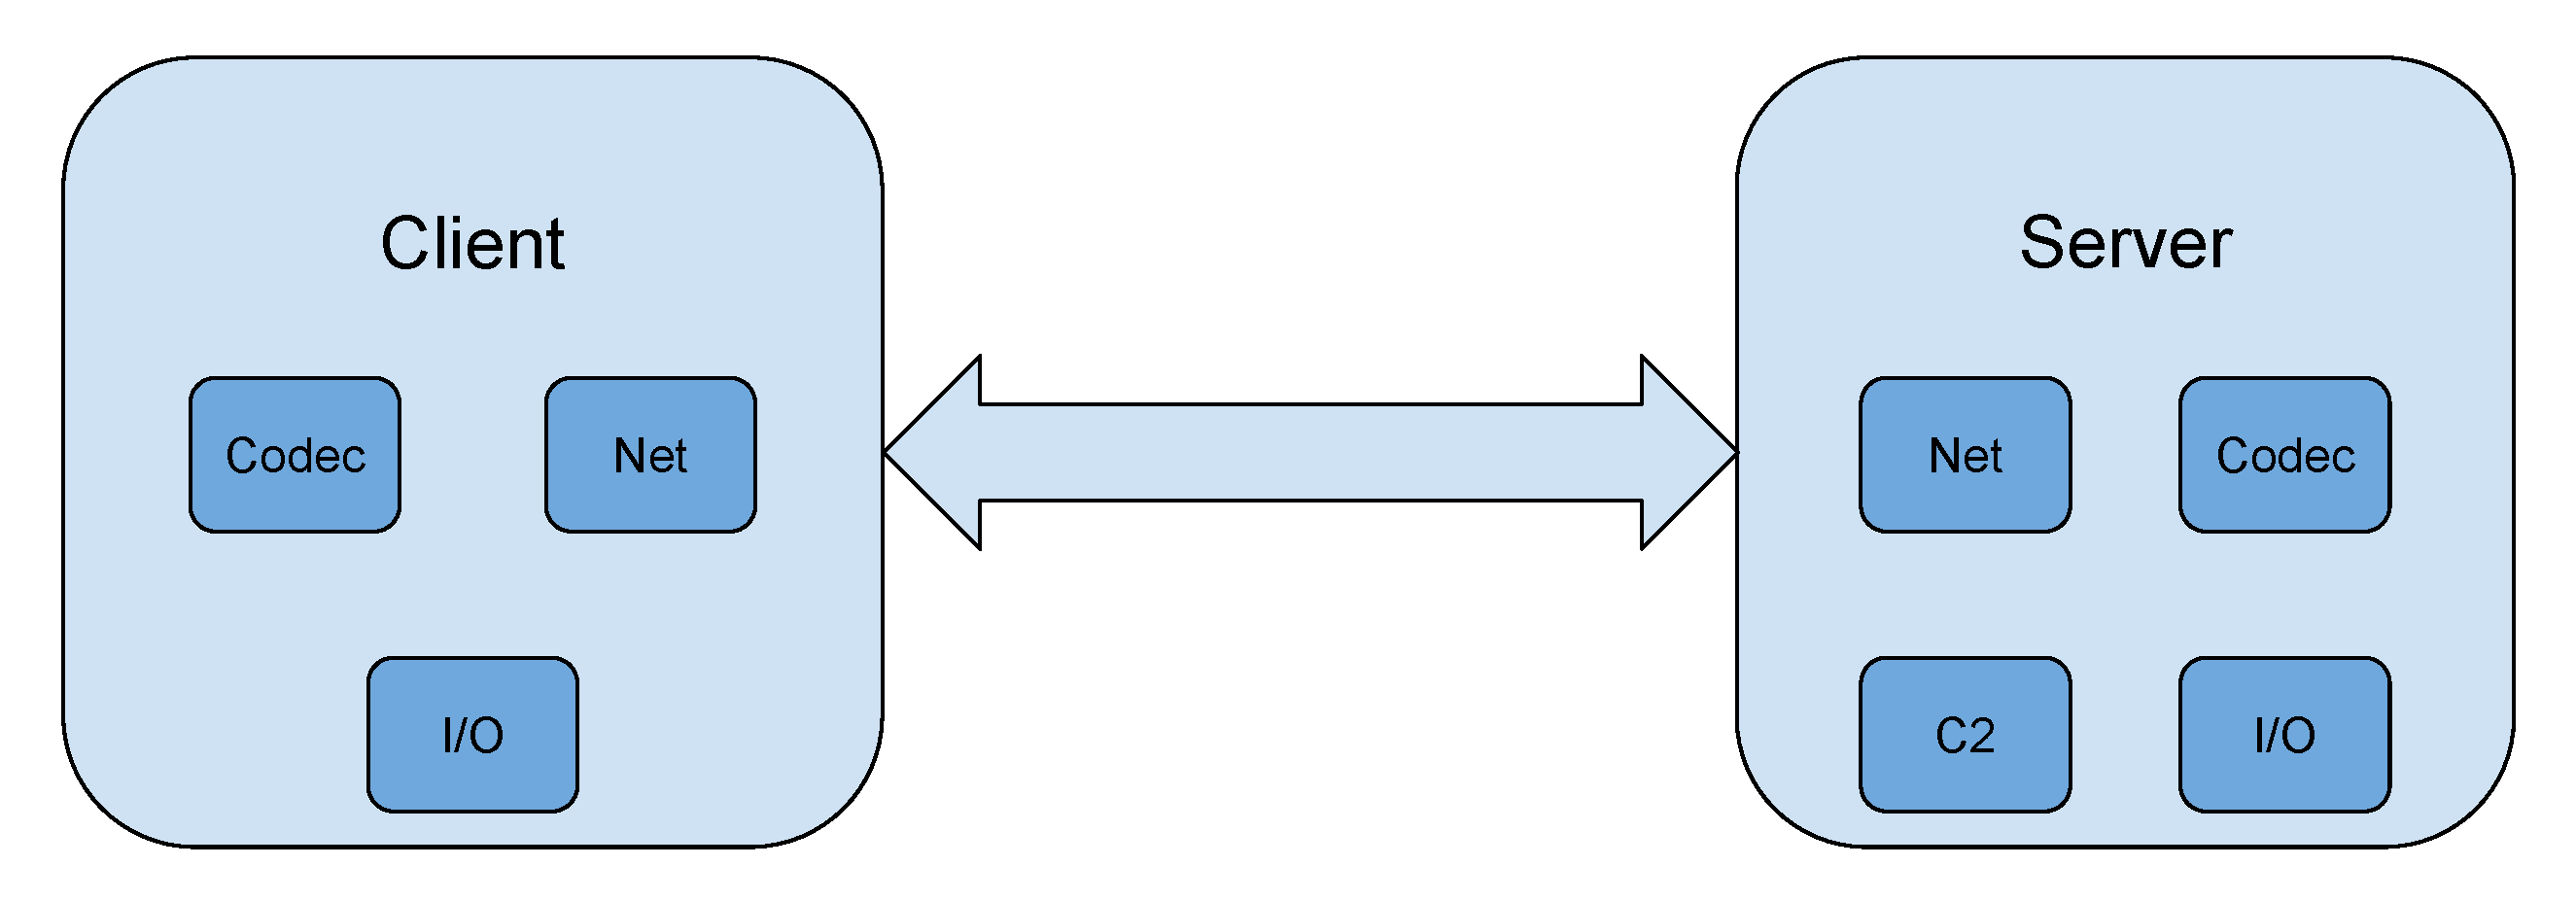
\includegraphics[width=0.5\textwidth]{img/client-server-architecture}
  \caption{Client-Server Model for Covert Communication}
  \label{fig:architecture}
\end{figure}

The server is designed similarly to the client, but features on suplimentary
and critical component, namely the C2 module, which is responsible for command
and control. The control aspect represents user authentication and changing
UID and GID if necessary. The command aspect passes the input received from the
user and attempts to run it as a command, retrieve the output and pass it to the
Codec component.

The way in which our useful data is encoded relies on the options field in the
TCP Header, as outlined in Figure \ref{fig:tcp-header}. The maximum supported
length is 320 bits, or 40 bytes. Most options follow a TLV\footnote{Type, Length, Value}
format. However, routers are known to drop packets with unrecognized options.
Consequently, our solution appears to send a valid TCP option. For this
purpose we use the TCP Alternate Checksum Data option which allows us to
dedicate 37 bytes for useful data, and 3 bytes for TCP options metadata.
This ensures both maximal utilization of the TCP options field and adequate
behavior from intermediary routing equipment.

\begin{figure}
  \centering
  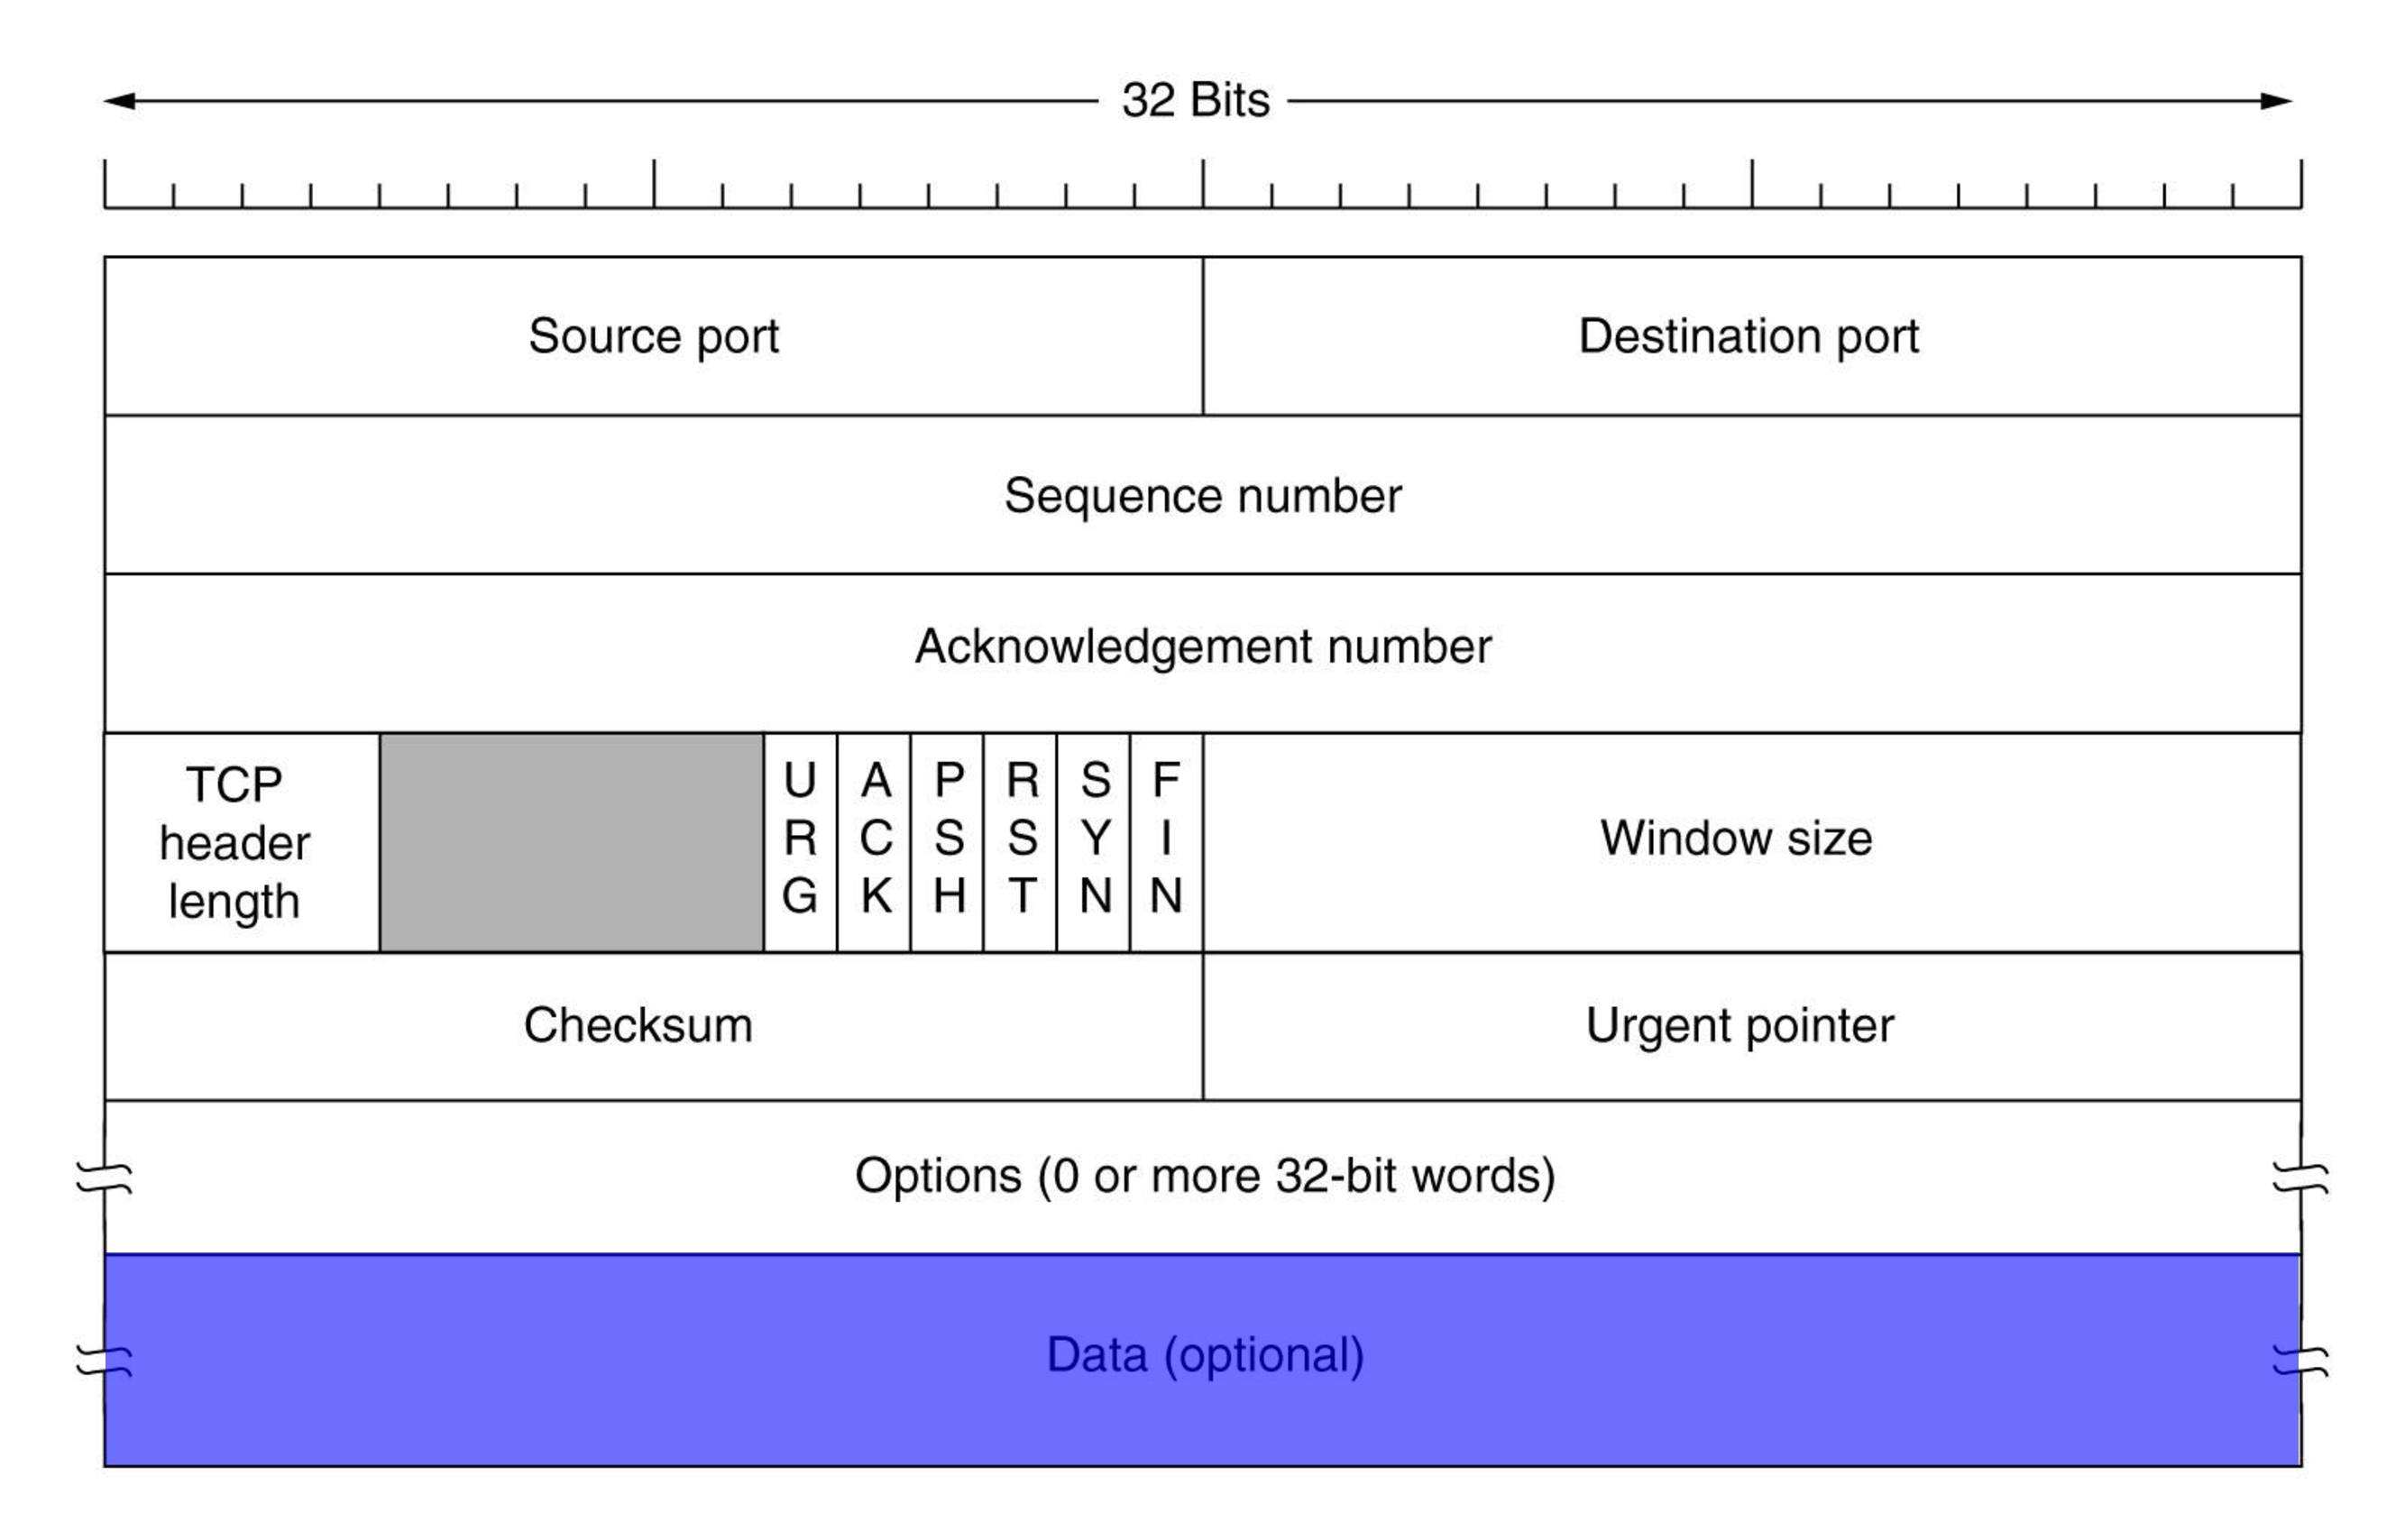
\includegraphics[width=0.5\textwidth]{img/tcp-header}
  \caption{TCP Header}
  \label{fig:tcp-header}
\end{figure}


\section{Implementation}
\label{sec:implementation}
% vim: set tw=78 sts=2 sw=2 ts=8 aw et ai:
Having provided an overview on how our solution is designed and how it should
behave, we will now describe the implementation details and obstacles we have
come across. We have implemented a client and a server which hide application
level data in the TCP options field and use it as a command-line interface to
a remote system. We have decided to implement this for Linux systems due to
the fact the Linux system programming interface is extremely flexible and easy
to comprehend.

\subsection{Input and Output}


The I/O module has two functions : getting the input from the user and printing
the response from the server after decoding.

For the input fetching, we assume that the user wants to run multiple commands
on the remote server or send a script/config file to the server. For the first
scenario, we will have an infinite loop that will read each command, send it to 
the Codec module and wait for response. As soon as the user inputs the "quit"
command, the session is terminated.

\begin{lstlisting}[caption={Basic command processing},
                   label={lst:our-tcphdr},
                   basicstyle=\footnotesize,
                   captionpos=b,
                   frame=single,
                   language=C
                  ]

while(1){
  Get command for stdin;
  if command == "quit"
    break;
  Send command to Codec;
  Wait for answer;
  Print answer;
}
\end{lstlisting}

If the user chooses to send a script or a config file to the server, we must open
the given file, send each line to the Codec module (which must first notify the server 
that a file is being sent) and then ask the user what the next action will be. At this
point, the user can choose to either terminate the session, send another file or send 
commands. 

\begin{lstlisting}[caption={File processing},
                   label={lst:our-tcphdr},
                   basicstyle=\footnotesize,
                   captionpos=b,
                   frame=single,
                   language=C
                  ]


  Get file for stdin;
  Open file;
  while (not end of file)
    Send each line to Codec;
  Prompt user for next action;
  if "quit"
    End session;
  elseif "continue"
    Send new file (goto first step);
  else
    Send commands (goto while(1));

\end{lstlisting}

Result printing is only present if the sent command had actual output. If not, nothing will
be printed and the user will be prompted for the next command. The file transfer will not 
generate output.



\subsection{Information Encoding}

Another module of our project is represented by the Encoding module. As we
have previously mentioned, the TCP header options field offers us 37 useful
bytes. Although this is a greater capacity than other protocols offer, it is
still a limited amount, so we have to use it properly.

The first thing to do is minimize the size of the input data (the useful
data encapsulated inside the TCP header), which leads to the idea of compressing
it. Our communication must be reliable and entirely exact, pointing to an
approach based on a lossless data compression algorithm. One of the most
suitable lossless algorithms is Huffman coding.

Huffman coding\cite{huffman1952method} is an entropy encoding algorithm using
a variable-length code table for encoding source symbols (characters in the
current situation), where the table is generated based on the probabilities of
occurence for each of the source symbols. In the end, what you get is a binary
tree of nodes which provides you unique combinations of bits for all the
symbols.

Practically speaking, the compression technique works in the following way:
first, all the nodes are leaf nodes, which contain the symbol itself and the
frequency of occurence; then the nodes are taken two by two starting with the
smallest frequencies, joining them by a common parent containing the sum of
their frequencies; the process is repeated until you have a single root node;
the edges are given bit values (0 the left branches, 1 the right branches);
the encoding for each letter is calculated by following the path of bits from
the root to the corresponding leaf.

\begin{figure}
  \centering
  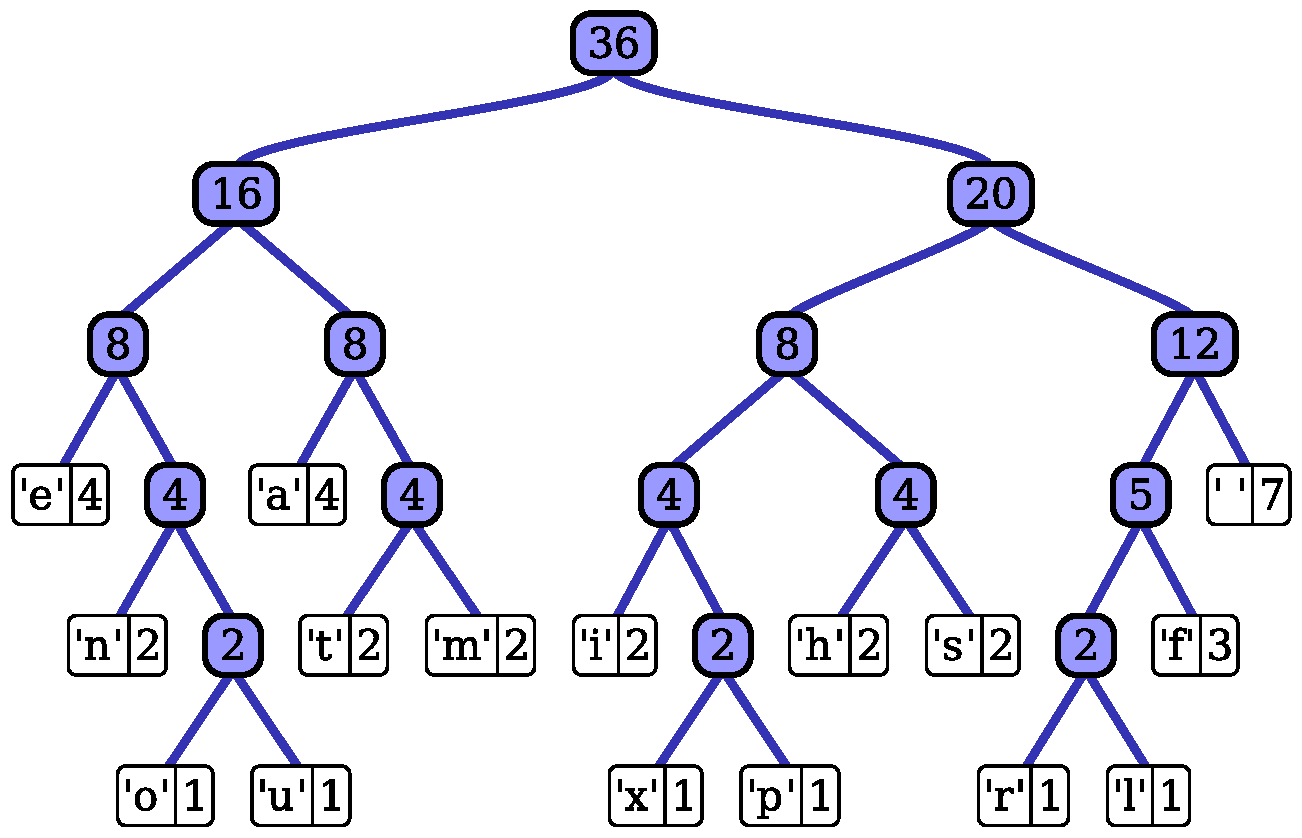
\includegraphics[width=0.5\textwidth]{img/huffman}
  \caption{Huffman tree generated for "this is an example of a huffman tree"}
  \label{fig:huffman}
\end{figure}

Reffering to the example in Figure \ref{fig:huffman}, the code for 'e' would
be '000', for 'a' '010', for 'u' '00111', and so on. As you can see, the most
frequent characters have the shortest codes.

In order to create a working encoding module, we have implemented the Huffman
algorithm to encode / compress the payload of our message. The result is a
sequence of bits to be added in the 37 bytes left of the options field.

But the things weren't that simple. First of all, the message had to be decoded
when it arrived at the destination. For this to be accomplished, we needed to
send the codebook along with the encoded message, so the first bytes of the
field had to define the length of the codebook and describe the codebook itself.

Another problem to overcome was that the commands given through our protocol
could easily exceed the size of a single TCP options field, considering the
codebook and its description included. This was solved by giving each command
a unique identificator, splitting the message and adding the identificator to
each resulting part.

To be continued here with a scheme of how the message looks like after encoding,
compressing and splitting.

\subsection{Network Communication}

After the Codec module splits the query or response and applies compression,
data is passed to the Net module, which is responsible for encapsulating it in
the TCP header and sending it to the other endpoint.

\begin{lstlisting}[caption={Default TCP Header Structure},
                   label={lst:def-tcphdr},
                   basicstyle=\footnotesize,
                   captionpos=b,
                   frame=single,
                   language=C
                  ]
typedef struct __attribute__ ((packed)) tcphdr {
     uint16_t th_sport;
     uint16_t th_dport;
     uint32_t  th_seq;
     uint32_t  th_ack;
 #ifndef __BIG_ENDIAN__
 #ifdef __IMAGECRAFT__
     unsigned th_x2:4,
              th_off:4;
 #else /* #ifndef __BIG_ENDIAN__ */
     uint8_t  th_x2:4,
             th_off:4;
 #endif
 #else /* #ifndef __BIG_ENDIAN__ */
     uint8_t  th_off:4,
             th_x2:4;
 #endif
     uint8_t  th_flags;
     uint16_t th_win;
     uint16_t th_sum;
     uint16_t th_urp;
} TCPHDR;
\end{lstlisting}

Using conventional Linux sockets will not be an option in our case. By default,
neither datagram, nor stream sockets provide sufficient functionality. While the
address and ports can be specified by the programmer, there is no manner to
configuring TCP options. Additionally, the structure that represents the TCP header
in the system libraries provides specific fields only for popular TCP attributes,
and no representation for TCP options, which are the key component of our
steganographic solution. The scarcity of individual configurable fields can be
observed in Listing \ref{lst:def-tcphdr}.

Consequently, we have opted to use raw sockets for our purposes. In terms of
network programming, raw sockets allow for Internet Protocol packets to be sent,
without any transport protocol information. System utilities such as ping and
traceroute make use of raw sockets since they rely on ICMP. We will not be
implementing a new transport protocol, nor will we use ICMP, but rather we will
use a more verbose variant of TCP, one which allows us to configure and
encapsulate TCP options into the TCP header. As a result, our implementation
makes use of a detailed TCP header, as can be seen from Listing \ref{lst:our-tcphdr}.

\begin{lstlisting}[caption={Verbose TCP Header Structure},
                   label={lst:our-tcphdr},
                   basicstyle=\footnotesize,
                   captionpos=b,
                   frame=single,
                   language=C
                  ]
struct tcp_header {
  uint16_t  srcp;    /* Source port */
  uint16_t  dstp;    /* Destination port */
  uint32_t  seqn;    /* Sequence number */
  uint32_t  ackn;    /* Acknowledgement number */
  uint16_t  ns:1;    /* ECN nonce concealment */
  uint16_t  res:3;   /* Reserved */
  uint16_t  doff:4;  /* Data offset */
  uint16_t  fin:1;   /* No more data from sender */
  uint16_t  syn:1;   /* Sync sequence numbers */
  uint16_t  rst:1;   /* Reset the connection */
  uint16_t  psh:1;   /* Push function. */
  uint16_t  ack:1;   /* Indicates ackn is relevant */
  uint16_t  urg:1;   /* Indicates urgp is relevant */
  uint16_t  ece:1;   /* Explicit congestion */
  uint16_t  cwr:1;   /* Congestion window reduced */
  uint16_t  win_sz;  /* Window size */
  uint16_t  chksum;  /* Checksum */
  uint16_t  urgp;    /* Last urgent data byte */
  char      opts[MAX_TCP_OPTS_LEN]; /* TCP options */
};
\end{lstlisting}

There is a drawback to using raw sockets, however. The usage of raw sockets
requires either having an effective UID of 0 or the CAP_NET_RAW capability.
While using capabilities allows for fine-grained control of privileges, requesting
that the program is run as root and dropping privileges when actually executing
commands is an equivalent approach. The above-mentioned utility ping also
runs as root.

In order for our implementation not to incur the attention of firewall, IDS and
IPS systems, a session between the endpoints should look as similar as possible
to a normal TCP communication. The TCP semantics must be preserved and we must
use a TCP option that is valid such that it can be accepted by intermediary
devices, yet allows us to encapsulate application level data. Thankfully, there
is such an option. RFC1146 \cite{rfc1146} describes options for extended checksum
information: TCP Alternate Checksum Request and TCP Alternate Checksum Data.

The TCP Alternate Checksum Request option is used to negociate usage of extended
checksum information between peers and is considered a prerequisite before actually
using the extended checksum. We perform this negociation during the three-way
handshake normally used by TCP communication. While this does not transfer any
useful data, it aids in simulating a proper TCP communication with extended
checksum information, thus thwarting analysis by a firewall or network administrator.

The TCP Alternate Checksum Data option is paramount to our goals. The only
resctrictions that apply to it is that the length specified in the TCP option
matches the actual data length. Other aspects such as whether it replaces or
supplements normal TCP checksum data, or what the algorithm used to compute the
checksum is are not enforced. Therefore, the value of this TCP option does not
have a distinguishable pattern to abide by, making it perfect for sending data.

There is a small note to be made with regards to intermediary networking devices.
Researchers of the Multipath TCP protocol \cite{mptcp-how-hard} also use TCP options, but
their goal is to pass metadata which is specific to a new protocol. Nevertheless,
they have identified issues with routing equipment, named middleboxes in their work,
which could interfere with our solution as well:
\begin{itemize}
\item Segment splitting
\item Segment coalescing
\item Removing TCP options
\item Dropping packets with unknown TCP options
\end{itemize}

Segment splitting and segment coalescing would not cause issues with our implementation
since, as long as the data arrives in order, which is what TCP does, the useful
information is not corrupted and can pe properly reassembled.

The removal of TCP options and the fact that packets with unknown options can be
droppend however can be damaging to our system, since it would act as a denial of
service. Requests would not reach the server and neither would replies be passed
back to the client. A study of networking equipment, the options they support, their
behavior with regards to unknown TCP options and how common they can be found in
the Internet is beyond the scope of this paper however.

\subsection{Command and Control}

The Command and Control module, C2 in short, is exclusive to the server and it is
employed to handle any of the set of commands sent by the client, together with additional
system settings that might be required. In the architectural view, the C2 module
communicates with the Codec module. The Codec module provides the C2 module with
its input, i.e. the string that results after the decompressing and decoding stages
have been successfully performed and receives from the C2 module the output, i.e.
the command results.
	
The "command" section of the C2 module is responsible with two important operations:
\begin{itemize}
\item Setting the UID and the GID before attempting to execute the command \\
The server runs with root privileges on the destination machine in order to be
able to create the raw sockets which are needed to establish the TCP communication
link. Naturally, to avoid security breaches we do not wish to allow any potentially
harmful remote user to run commands as root and therefore we create a specific
account with normal or carefully customized privileges. This account will be used
to run the given commands. The command submodule accomplishes this step by setting
the UID and the GID as appropriate.
\item Resetting the uid and gid back to their original values \\
After the command is executed, the command submodule restores the original state
of the UID and GID by using the setresuid() and setresgid() functions provided by glibc.
\end{itemize}

The "control" section is responsible with the effective execution of the received
command. Due to security concerns, we do not blindly execute the command even if
we have previously set the UID and GID. Instead we have implemented a command parser
to extract the tokens and the operands from the given string, which are then
analyzed for safety. The module supports:
\begin{itemize}
\item external commands with multiple arguments
\item internal shell commands (such as cd)
\item redirects (>, <, $\gg$, 2\&> and so on)
\item pipes
\item sequential/parallel command operators (such as ;, | and \&)
\item conditional command operators (\&\&, ||) 
\end{itemize}

This implementation guarantees correct priority of operators in accordance with
shell rules and also supports setting and reading environment variables.
If the submodule has detected an unsafe or unsupported operation request,
an error message is generated.

After the command is executed, the control submodule reads from stdin and stderr
and passes the output back to the Codec module, which will compress and encode
it into as many packets as it is necessary.



\section{Experimental Setup}
\label{sec:setup}
% vim: set tw=78 sts=2 sw=2 ts=8 aw et ai:

In order to define recursion, one must first define recursion.


\section{Scenarios and Results}
\label{sec:results}
% vim: set tw=78 sts=2 sw=2 ts=8 aw et ai:

Having described our test environment, the current section will present the
results of our three scenarios illustrated above.

When testing locally using two loopback addresses our connection is ideal.
There is no intermediary networking equipment that can interfere with our
custom traffic. Our covert communication succeeds and we are able to send
commands successfully, while adhering to restrictions such as limited capacity
per packet and prohibition to run privileged commands.

\begin{figure}
  \centering
  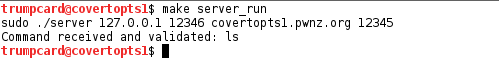
\includegraphics[width=0.5\textwidth]{img/server-run}
  \caption{Server Side Session}
  \label{fig:server-run}
\end{figure}

\begin{figure}
  \centering
  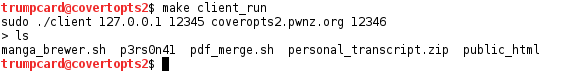
\includegraphics[width=0.5\textwidth]{img/client-run}
  \caption{Client Side Session}
  \label{fig:client-run}
\end{figure}

The second test we performed is whether a modern firewall equipment handles
our covert session differently. As can be seen from Figure
\ref{fig:server-run} and Figure \ref{fig:client-run}, Cisco ASA does not strip
or drop packets which use the TCP Alternate Checksum Data option. The
hostnames are conveniently set to illustrate the two endpoints. It is worth
mentioning that we could not explore the full range of options such a
dedicated device offers, but we found no explicit feature that affects TCP
options directly.

Finally, we considered a real world test, between two public IPs. Despite our
previous tests being encouraging, we could not replicate the results in a real
world scenario. Since the intermediary devices are not under our control, we
cannot be certain that the root cause is explicit filtering of certain TCP
options or simply a default behaviour like the ones described in Subsection
\ref{sec:net-comm}. We cannot even determine the hardware platform of these
devices in order to speculate as to their prevalence on the Internet.

Overall, our solution has the capability to be deployed in real life, but its
effectiveness is highly dependent on the behavior of networking equipment
found between endpoints.


\section{Conclusion and Further Work}
\label{sec:conclusion}
% vim: set tw=78 sts=2 sw=2 ts=8 aw et ai:

Evolution of today's computer science demands increasingly new and intelligent
approaches. Steganography is a field with a very long history. Starting from
the antique wax tablets, continuing with invisible ink, steganography has also
evolved, so that nowadays we can speak of digital steganography.

Our project successfully adds up to this research direction. We have managed to
implement a novel approach, we have a working steganographic communication and,
as far as we know, the biggest amount of hidden data transmitted inside a
single segment. We have used the TCP header, more precisely the "Options"
field, sending a total of 37 bytes per TCP segment.

As future work, we would like to follow a few directions. First, we would like to
see how the application behaves in a controlled, larger system, so that we may solve
the problems that occured when we tried to send packets between two public IPs. If
the problem is related to devices not supporting the extra options field, we might 
consider sending packets to intermediate stations, on paths that we know are safe
and will not cause those packets to be dropped. Second, as you have seen, using
Huffman encoding took us a large number of bytes to assure the necessary metadata
(codebook, message length, etc). Future studies will include finding and
implementing better compression algorithms to minimize the size of the
communication. Third, cryptography will be a future thing to be added for
improved security, in order to add a new level of hiding to our steganographic data.


\section*{Acknowledgment}
\label{sec:acknowledgment}

The authors would like to thank XYZ for their support and dedication.

\bibliographystyle{abbrv}
\bibliography{my-paper}

\end{document}
